Es en esta fase donde delimitaremos los alcances y límites del problema en
función de su aplicabilidad final. También nos otorgará un marco de referencia
para delimitar el espacio de soluciones a buscar. Conocer el espacio de
soluciones incluye la identificación de las disposiciones prácticas de la
solución, por ejemplo, favorecer modelos ligeros si la solución se desplegará en
situaciones con bajo poder computacional como en dispositivos móviles, si la
solución va a automatizar o a asistir en la toma de decisiones, si va a
reemplazar una solución ya existente generar políticas para substitución y
reemplazo; así como todo el acervo del dominio que guiará el diseño de la
solución. El trabajo necesario para realizar un análisis genera surge de los dos
capítulos anteriores, donde se definió el problema, sus características y
propuestas de solución.

\subsection{Definir el problema bajo el dominio}

El problema a resolver es la detección de células glandulares en una laminilla
preparada de un \hyperlink{abbr}{PAP} para su posterior clasificación en
células normales, anormales y las clases en las que se dividen ambas categorías.

Es por ello que sabemos que debemos utilizar imágenes para resolver el problema.
Soluciones anteriores se basaban en la extracción de características de estas
imágenes para luego entrenar un algoritmo con datos tabulares recopilados y
empatados con las características extraídas de las imágenes. Esta fase de
extracción de características rápidamente se convertía en el eslabón más débil
de la solución debido a su dificultad y la baja capacidad de generalización. Es
por ello que se propuso trabajar con algoritmos de aprendizaje jerárquico,
capaces de aprender por si solos las características morfológicas que
diferencian una célula normal de una anormal.

El sistema se usará dentro de un laboratorio, por lo que la solución debe ser
optimizada para su implementación en un sistema embebido, debido a que un
laboratorio citológico es un lugar con restricción en recursos computacionales.
Así mismo, debe ser de bajo costo, por lo que nos hemos decantado por mantener
la solución dentro del dominio del software y hardware libres.

Los expertos consultados determinaron que el sistema incidirá en una etapa del
proceso de diagnóstico de cáncer específica, se determinó que el proceso
iterativo para generar la solución debe de comenzar primero clasificando a las
células en normal y anormal (en el análisis pre-diagnóstico realizado por el
cito-tecnólogo), para su posterior generalización a las categorías de
diagnóstico que se utilizan en la siguiente etapa del proceso de diagnóstico,
cuando la laminilla se envía al patólogo. Así mismo, se generó el supuesto de
que el núcleo celular contiene suficiente información para determinar si la
célula es normal o anormal, por lo que los algoritmos de preprocesamiento se
centrarán en esta característica.

\subsection{Búsqueda de soluciones previas}

Aparte de las soluciones expuestas en el Estado del Arte de esta tesis. Damos un
ejemplo de la primera aplicación de \hyperlink{abbr}{RNA} a la problemática y
como esta solución llegó a sobrepasar por mucho el rendimiento de las formas
tradicionales de análisis citológico. 

PAPNET es un sistema creado por la empresa Neuromedical Systems que utiliza una
RNA tradicional para detectar células anormales en un \hyperlink{abbr}{PAP}. Fue
la primera compañía en utilizar \hyperlink{abbr}{RNA} a la citología. Tiene una tasa FNR de 3\% lo
que la hace mejor que cualquier análisis tradicional de laboratorio, esto fue
comprobado gracias a un estudio de análisis clínico que realizaron; por lo que
fue el sistema más eficaz de antes del 2000 \cite{DeCresce1991}.

El problema con PAPNET era el costo. La diferencia con de su rendimiento con
respecto a las formas tradicionales era significativo pero no podía justificar
el costo 30 veces más elevado. El \hyperlink{abbr}{PAP} es un examen que se
tiene que repetir muchas veces en un mismo paciente a lo largo de su vida por lo
que pagar mucho es totalmente impráctico \cite{Media}. 

\subsection{Determinar tipo de problema}

Decidir si una célula es normal o anormal a partir de una imagen, es un problema
de clasificación. Sin embargo, existen diferentes maneras de abordar el
problema. Existen cuatro formas de aplicar el \hyperlink{abbr}{DL} a las
imágenes, por lo cual podemos proceder de las siguientes maneras (\autoref{fig:tipos}):

\begin{itemize}
    \item{\textbf{Clasificación:}} De una imagen que contiene una sola célula,
    determinar si es normal o anormal.
    \item{\textbf{Detección:}}: De una imagen que contiene varias células,
    determinar si cada una de ellas es normal o anormal.
    \item{\textbf{Segmentación semántica:}} De una imagen que contiene una o
    varias células, determinar si cierto pixel en particular pertenece a una
    célula normal, anormal o al fondo.
    \item{\textbf{Instanciación:}} De una imagen que contiene una o varias
    células, determinar si cierto pixel en particular pertenece a una célula
    normal, anormal o al fondo, diferenciando cada célula individual de las
    demás. 
\end{itemize}

\begin{figure}[H]
  \centering
  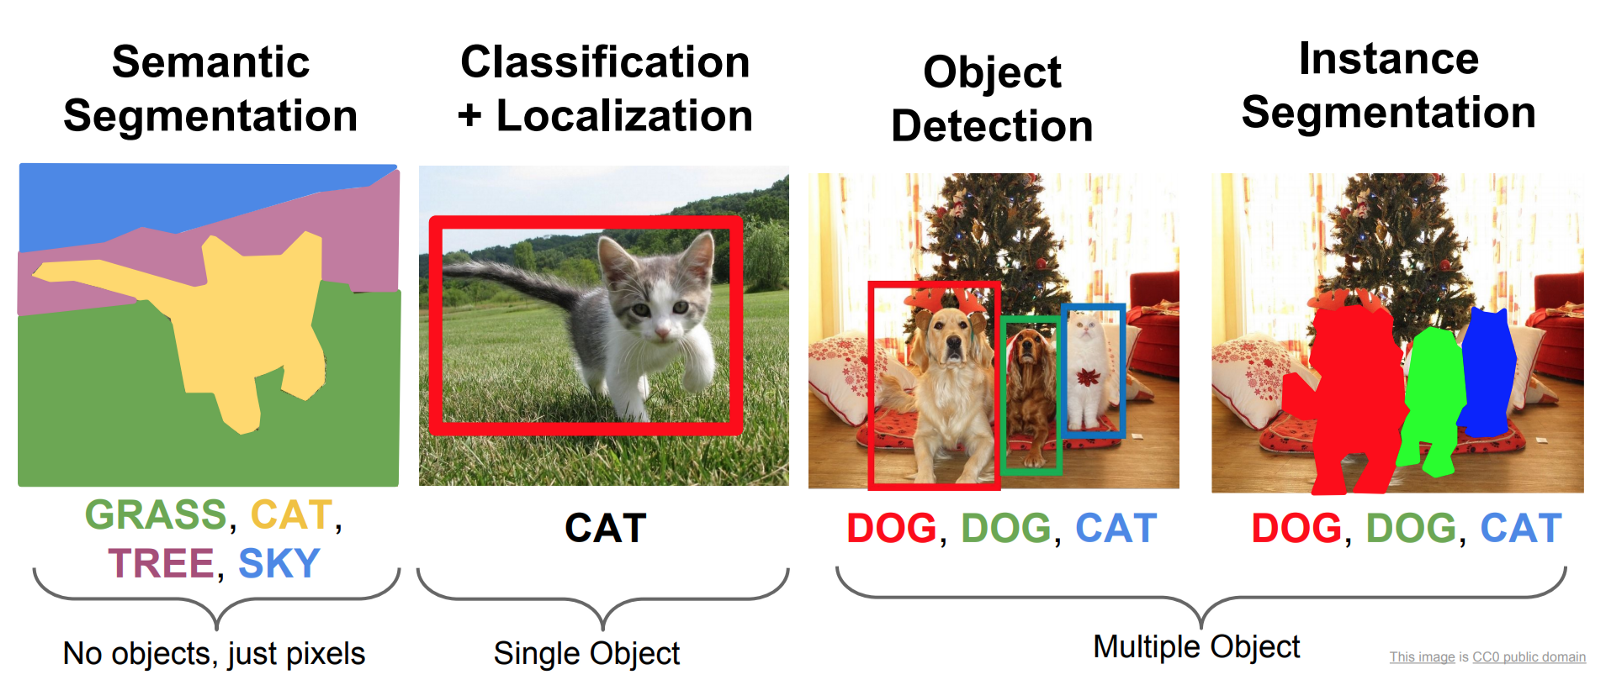
\includegraphics[width=0.8\textwidth]{capitulo_sdac/tipos}
  \caption{Tipos de visión por computadora eon Deep Learning}\label{fig:tipos}
\end{figure}


Como veremos posteriormente, por las características de la \hyperlink{abbr}{BD},
nos limitaremos a Clasificación y Segmentación semántica, sin embargo, a futuro
será provechoso implementar las otras técnicas para mejorar la funcionalidad del
sistema final.

Las métricas de rendimiento se basan no solo en métricas de clasificación de
imágenes, como el F1-score, Recall o la exactitud, sino también en la tasa de
falsos positivos, falsos negativos así como métricas que conjuguen ambos
concentos como la especificidad y la sensibilidad. Como se explicó en el
capítulo anterior. También se fijó el grado mínimo que tendrán estas métricas,
quedando en 95\%.

El problema de clasificación de imágenes ha tenido grandes avances en los
últimos tres años debido a las nuevas arquitecturas de
\hyperlink{abbr}{ConvNet}, por lo que estas se convertirán en el algoritmo
elegido, del cual probaremos varias arquitecturas. Basándonos en el buen
rendimiento que han tenido estas arquitecturas y haciendo uso de
\hyperlink{abbr}{TL}, exploramos soluciones previas y generales para potenciar
nuestro sistema particular, por lo que nos basaremos en ellas para alcanzar los
niveles de tolerancia requeridos.

\subsection{Generación de supuestos}

Los supuestos para llevar a cabo los experimentos de clasificación de imágenes
fueron los siguientes:

\begin{itemize}
  \item El núcleo celular contiene suficiente información para diferenciar entre
  los tipos de célula citológica cervical.
  \item Las técnicas de aumento de datos no inciden en la decisión del
  algoritmo.
  \item La red neuronal es capaz de diferenciar correctamente en un espacio
  multidimensional entre los tipos de célula.
\end{itemize}

El primer supuesto está presente en el desarrollo de los algoritmos de
aumentación de datos y la premisa que sustenta la investigación. Debido a la
dificultad para segmentar y extraer cada célula individual de una célula,
limitarnos al análisis del núcleo nos permite solventar un poco esta restricción
enfocándonos en la región más significativa de las que componen cualquier
célula. 

El segundo tiene que ver específicamente con las características de la imagen
aumentada; se requiere saber si los pixeles extras añadidos a la imagen en el
proceso de rotación afecta la inferencia del algoritmo o incide con ruido en la
decisión.

El tercero relaciona el espacio multidimensional generado por el algoritmo en
las capas convolucionales finales con una representación bidimensional para
visualizar como el algoritmo separa y agrupa las distintas clases del problema.
Con el objetivo de corroborar las métricas de clasificación.

\subsection{Propuesta}

La propuesta se define como: Un \hyperlink{abbr}{SDAC} basado en
\hyperlink{abbr}{DL} y \hyperlink{abbr}{ConvNet}s capaz de ser desplegado en
laboratorio, de bajo costo y con facilidad de uso. Que pueda clasificar células
en normales y anormales con un rendimiento aceptable.

La propuesta debe cumplir todos los objetivos planteados en esta tesis; para
generar un diseño conceptual y posterior prototipo para desplegarlo en una
solución al usuario final en trabajos posteriores.
